% Options for packages loaded elsewhere
\PassOptionsToPackage{unicode}{hyperref}
\PassOptionsToPackage{hyphens}{url}
\PassOptionsToPackage{dvipsnames,svgnames,x11names}{xcolor}
%
\documentclass[
  letterpaper,
  DIV=11,
  numbers=noendperiod]{scrreprt}

\usepackage{amsmath,amssymb}
\usepackage{iftex}
\ifPDFTeX
  \usepackage[T1]{fontenc}
  \usepackage[utf8]{inputenc}
  \usepackage{textcomp} % provide euro and other symbols
\else % if luatex or xetex
  \usepackage{unicode-math}
  \defaultfontfeatures{Scale=MatchLowercase}
  \defaultfontfeatures[\rmfamily]{Ligatures=TeX,Scale=1}
\fi
\usepackage{lmodern}
\ifPDFTeX\else  
    % xetex/luatex font selection
\fi
% Use upquote if available, for straight quotes in verbatim environments
\IfFileExists{upquote.sty}{\usepackage{upquote}}{}
\IfFileExists{microtype.sty}{% use microtype if available
  \usepackage[]{microtype}
  \UseMicrotypeSet[protrusion]{basicmath} % disable protrusion for tt fonts
}{}
\makeatletter
\@ifundefined{KOMAClassName}{% if non-KOMA class
  \IfFileExists{parskip.sty}{%
    \usepackage{parskip}
  }{% else
    \setlength{\parindent}{0pt}
    \setlength{\parskip}{6pt plus 2pt minus 1pt}}
}{% if KOMA class
  \KOMAoptions{parskip=half}}
\makeatother
\usepackage{xcolor}
\setlength{\emergencystretch}{3em} % prevent overfull lines
\setcounter{secnumdepth}{5}
% Make \paragraph and \subparagraph free-standing
\makeatletter
\ifx\paragraph\undefined\else
  \let\oldparagraph\paragraph
  \renewcommand{\paragraph}{
    \@ifstar
      \xxxParagraphStar
      \xxxParagraphNoStar
  }
  \newcommand{\xxxParagraphStar}[1]{\oldparagraph*{#1}\mbox{}}
  \newcommand{\xxxParagraphNoStar}[1]{\oldparagraph{#1}\mbox{}}
\fi
\ifx\subparagraph\undefined\else
  \let\oldsubparagraph\subparagraph
  \renewcommand{\subparagraph}{
    \@ifstar
      \xxxSubParagraphStar
      \xxxSubParagraphNoStar
  }
  \newcommand{\xxxSubParagraphStar}[1]{\oldsubparagraph*{#1}\mbox{}}
  \newcommand{\xxxSubParagraphNoStar}[1]{\oldsubparagraph{#1}\mbox{}}
\fi
\makeatother

\usepackage{color}
\usepackage{fancyvrb}
\newcommand{\VerbBar}{|}
\newcommand{\VERB}{\Verb[commandchars=\\\{\}]}
\DefineVerbatimEnvironment{Highlighting}{Verbatim}{commandchars=\\\{\}}
% Add ',fontsize=\small' for more characters per line
\usepackage{framed}
\definecolor{shadecolor}{RGB}{241,243,245}
\newenvironment{Shaded}{\begin{snugshade}}{\end{snugshade}}
\newcommand{\AlertTok}[1]{\textcolor[rgb]{0.68,0.00,0.00}{#1}}
\newcommand{\AnnotationTok}[1]{\textcolor[rgb]{0.37,0.37,0.37}{#1}}
\newcommand{\AttributeTok}[1]{\textcolor[rgb]{0.40,0.45,0.13}{#1}}
\newcommand{\BaseNTok}[1]{\textcolor[rgb]{0.68,0.00,0.00}{#1}}
\newcommand{\BuiltInTok}[1]{\textcolor[rgb]{0.00,0.23,0.31}{#1}}
\newcommand{\CharTok}[1]{\textcolor[rgb]{0.13,0.47,0.30}{#1}}
\newcommand{\CommentTok}[1]{\textcolor[rgb]{0.37,0.37,0.37}{#1}}
\newcommand{\CommentVarTok}[1]{\textcolor[rgb]{0.37,0.37,0.37}{\textit{#1}}}
\newcommand{\ConstantTok}[1]{\textcolor[rgb]{0.56,0.35,0.01}{#1}}
\newcommand{\ControlFlowTok}[1]{\textcolor[rgb]{0.00,0.23,0.31}{\textbf{#1}}}
\newcommand{\DataTypeTok}[1]{\textcolor[rgb]{0.68,0.00,0.00}{#1}}
\newcommand{\DecValTok}[1]{\textcolor[rgb]{0.68,0.00,0.00}{#1}}
\newcommand{\DocumentationTok}[1]{\textcolor[rgb]{0.37,0.37,0.37}{\textit{#1}}}
\newcommand{\ErrorTok}[1]{\textcolor[rgb]{0.68,0.00,0.00}{#1}}
\newcommand{\ExtensionTok}[1]{\textcolor[rgb]{0.00,0.23,0.31}{#1}}
\newcommand{\FloatTok}[1]{\textcolor[rgb]{0.68,0.00,0.00}{#1}}
\newcommand{\FunctionTok}[1]{\textcolor[rgb]{0.28,0.35,0.67}{#1}}
\newcommand{\ImportTok}[1]{\textcolor[rgb]{0.00,0.46,0.62}{#1}}
\newcommand{\InformationTok}[1]{\textcolor[rgb]{0.37,0.37,0.37}{#1}}
\newcommand{\KeywordTok}[1]{\textcolor[rgb]{0.00,0.23,0.31}{\textbf{#1}}}
\newcommand{\NormalTok}[1]{\textcolor[rgb]{0.00,0.23,0.31}{#1}}
\newcommand{\OperatorTok}[1]{\textcolor[rgb]{0.37,0.37,0.37}{#1}}
\newcommand{\OtherTok}[1]{\textcolor[rgb]{0.00,0.23,0.31}{#1}}
\newcommand{\PreprocessorTok}[1]{\textcolor[rgb]{0.68,0.00,0.00}{#1}}
\newcommand{\RegionMarkerTok}[1]{\textcolor[rgb]{0.00,0.23,0.31}{#1}}
\newcommand{\SpecialCharTok}[1]{\textcolor[rgb]{0.37,0.37,0.37}{#1}}
\newcommand{\SpecialStringTok}[1]{\textcolor[rgb]{0.13,0.47,0.30}{#1}}
\newcommand{\StringTok}[1]{\textcolor[rgb]{0.13,0.47,0.30}{#1}}
\newcommand{\VariableTok}[1]{\textcolor[rgb]{0.07,0.07,0.07}{#1}}
\newcommand{\VerbatimStringTok}[1]{\textcolor[rgb]{0.13,0.47,0.30}{#1}}
\newcommand{\WarningTok}[1]{\textcolor[rgb]{0.37,0.37,0.37}{\textit{#1}}}

\providecommand{\tightlist}{%
  \setlength{\itemsep}{0pt}\setlength{\parskip}{0pt}}\usepackage{longtable,booktabs,array}
\usepackage{calc} % for calculating minipage widths
% Correct order of tables after \paragraph or \subparagraph
\usepackage{etoolbox}
\makeatletter
\patchcmd\longtable{\par}{\if@noskipsec\mbox{}\fi\par}{}{}
\makeatother
% Allow footnotes in longtable head/foot
\IfFileExists{footnotehyper.sty}{\usepackage{footnotehyper}}{\usepackage{footnote}}
\makesavenoteenv{longtable}
\usepackage{graphicx}
\makeatletter
\def\maxwidth{\ifdim\Gin@nat@width>\linewidth\linewidth\else\Gin@nat@width\fi}
\def\maxheight{\ifdim\Gin@nat@height>\textheight\textheight\else\Gin@nat@height\fi}
\makeatother
% Scale images if necessary, so that they will not overflow the page
% margins by default, and it is still possible to overwrite the defaults
% using explicit options in \includegraphics[width, height, ...]{}
\setkeys{Gin}{width=\maxwidth,height=\maxheight,keepaspectratio}
% Set default figure placement to htbp
\makeatletter
\def\fps@figure{htbp}
\makeatother

\KOMAoption{captions}{tableheading}
\makeatletter
\@ifpackageloaded{bookmark}{}{\usepackage{bookmark}}
\makeatother
\makeatletter
\@ifpackageloaded{caption}{}{\usepackage{caption}}
\AtBeginDocument{%
\ifdefined\contentsname
  \renewcommand*\contentsname{Table of contents}
\else
  \newcommand\contentsname{Table of contents}
\fi
\ifdefined\listfigurename
  \renewcommand*\listfigurename{List of Figures}
\else
  \newcommand\listfigurename{List of Figures}
\fi
\ifdefined\listtablename
  \renewcommand*\listtablename{List of Tables}
\else
  \newcommand\listtablename{List of Tables}
\fi
\ifdefined\figurename
  \renewcommand*\figurename{Figure}
\else
  \newcommand\figurename{Figure}
\fi
\ifdefined\tablename
  \renewcommand*\tablename{Table}
\else
  \newcommand\tablename{Table}
\fi
}
\@ifpackageloaded{float}{}{\usepackage{float}}
\floatstyle{ruled}
\@ifundefined{c@chapter}{\newfloat{codelisting}{h}{lop}}{\newfloat{codelisting}{h}{lop}[chapter]}
\floatname{codelisting}{Listing}
\newcommand*\listoflistings{\listof{codelisting}{List of Listings}}
\makeatother
\makeatletter
\makeatother
\makeatletter
\@ifpackageloaded{caption}{}{\usepackage{caption}}
\@ifpackageloaded{subcaption}{}{\usepackage{subcaption}}
\makeatother

\ifLuaTeX
  \usepackage{selnolig}  % disable illegal ligatures
\fi
\usepackage{bookmark}

\IfFileExists{xurl.sty}{\usepackage{xurl}}{} % add URL line breaks if available
\urlstyle{same} % disable monospaced font for URLs
\hypersetup{
  pdftitle={Popular Songs on TikTok and Beyond},
  pdfauthor={Melanie Boleng},
  colorlinks=true,
  linkcolor={blue},
  filecolor={Maroon},
  citecolor={Blue},
  urlcolor={Blue},
  pdfcreator={LaTeX via pandoc}}


\title{Popular Songs on TikTok and Beyond}
\author{Melanie Boleng}
\date{2024-12-06}

\begin{document}
\maketitle

\renewcommand*\contentsname{Table of contents}
{
\hypersetup{linkcolor=}
\setcounter{tocdepth}{2}
\tableofcontents
}

\bookmarksetup{startatroot}

\chapter*{Goals and Data Sources}\label{goals-and-data-sources}
\addcontentsline{toc}{chapter}{Goals and Data Sources}

\markboth{Goals and Data Sources}{Goals and Data Sources}

The goal of this project is to explore the intersection of the top songs
on the social media platform TikTok and song charts (Spotify top songs,
and the Billboard Hot 100) for the year 2022. We are interested in
analyzing if top songs on TikTok made it to the charts, or vice versa.
We also plan to look at the tempo of the songs to identify any patterns
among high-tempo songs and ranking on charts.

The data sources include a dataset of top songs on TikTok, top Spotify
songs, and the Billboard Hot 100. All three charts rank songs in
slightly different ways as explained below.

\subsection{Spotify Dataset}

This dataset was found on Kaggle.The user who uploaded the data to
Kaggle used Spotify's API to scrape the data. The table features 17 rows
and 646 observations. The grain of the table is a song and its
attributes. As this data was retrieved from Spotify like the TikTok
dataset, the most relevant columns are the same: track\_name,
artist\_name, peak\_rank, and tempo. The peak\_rank column indicated the
highest the song climbed on the chart. A lower number indicated that the
song reached a higher ranking.

\begin{figure}[H]

{\centering 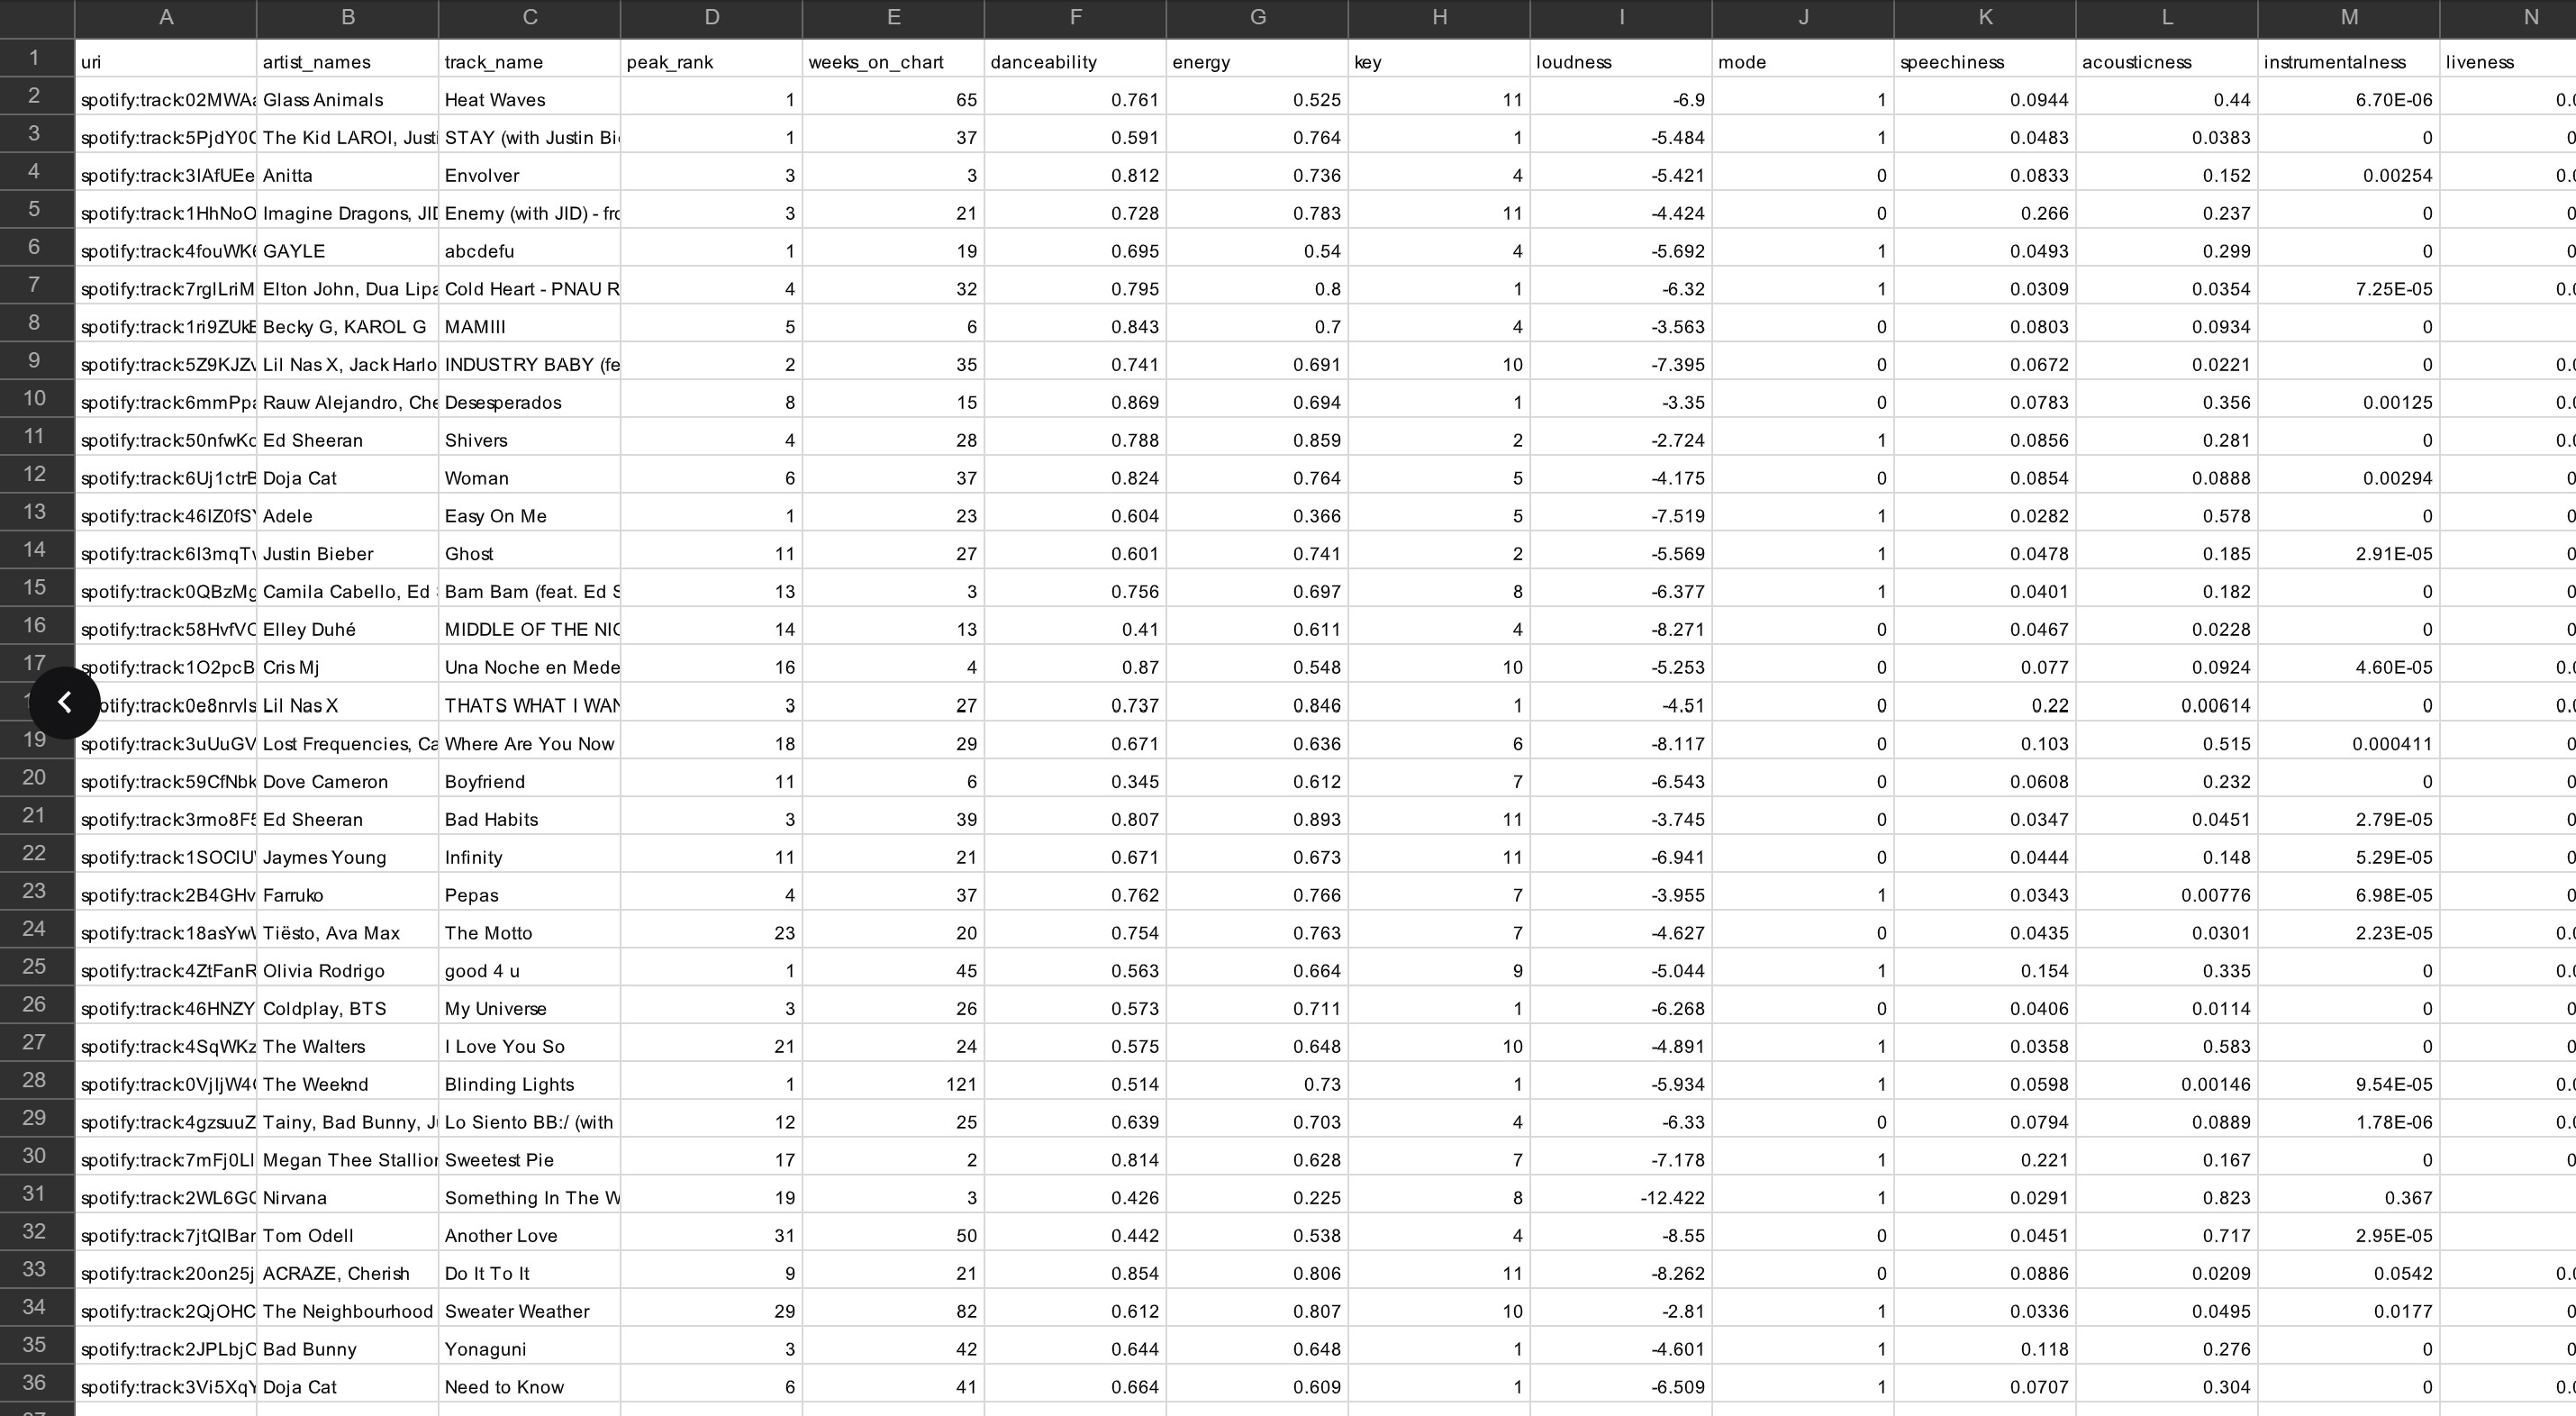
\includegraphics[width=5.82292in,height=\textheight]{images/spotify_songs_screenshot.jpg}

}

\caption{Top Songs on Spotify}

\end{figure}%

\subsection{TikTok Dataset}

This dataset was found on Kaggle. The user who uploaded this data to
Kaggle retrieved the data from a playlist on Spotify of trending songs
on TikTok. Spotify has an API that allows user to scrape data. This
table features 18 columns and 263 observations. The grain of the table
is a song and its attributes. The columns most relevant to our goals are
the track\_name, artist\_name, track\_pop, and tempo. The track\_pop
column represents the popularity of the song. The values in the column
are produced and used by Spotify's algorithm, with a higher number
indicating that the track was more popular.

\begin{figure}[H]

{\centering 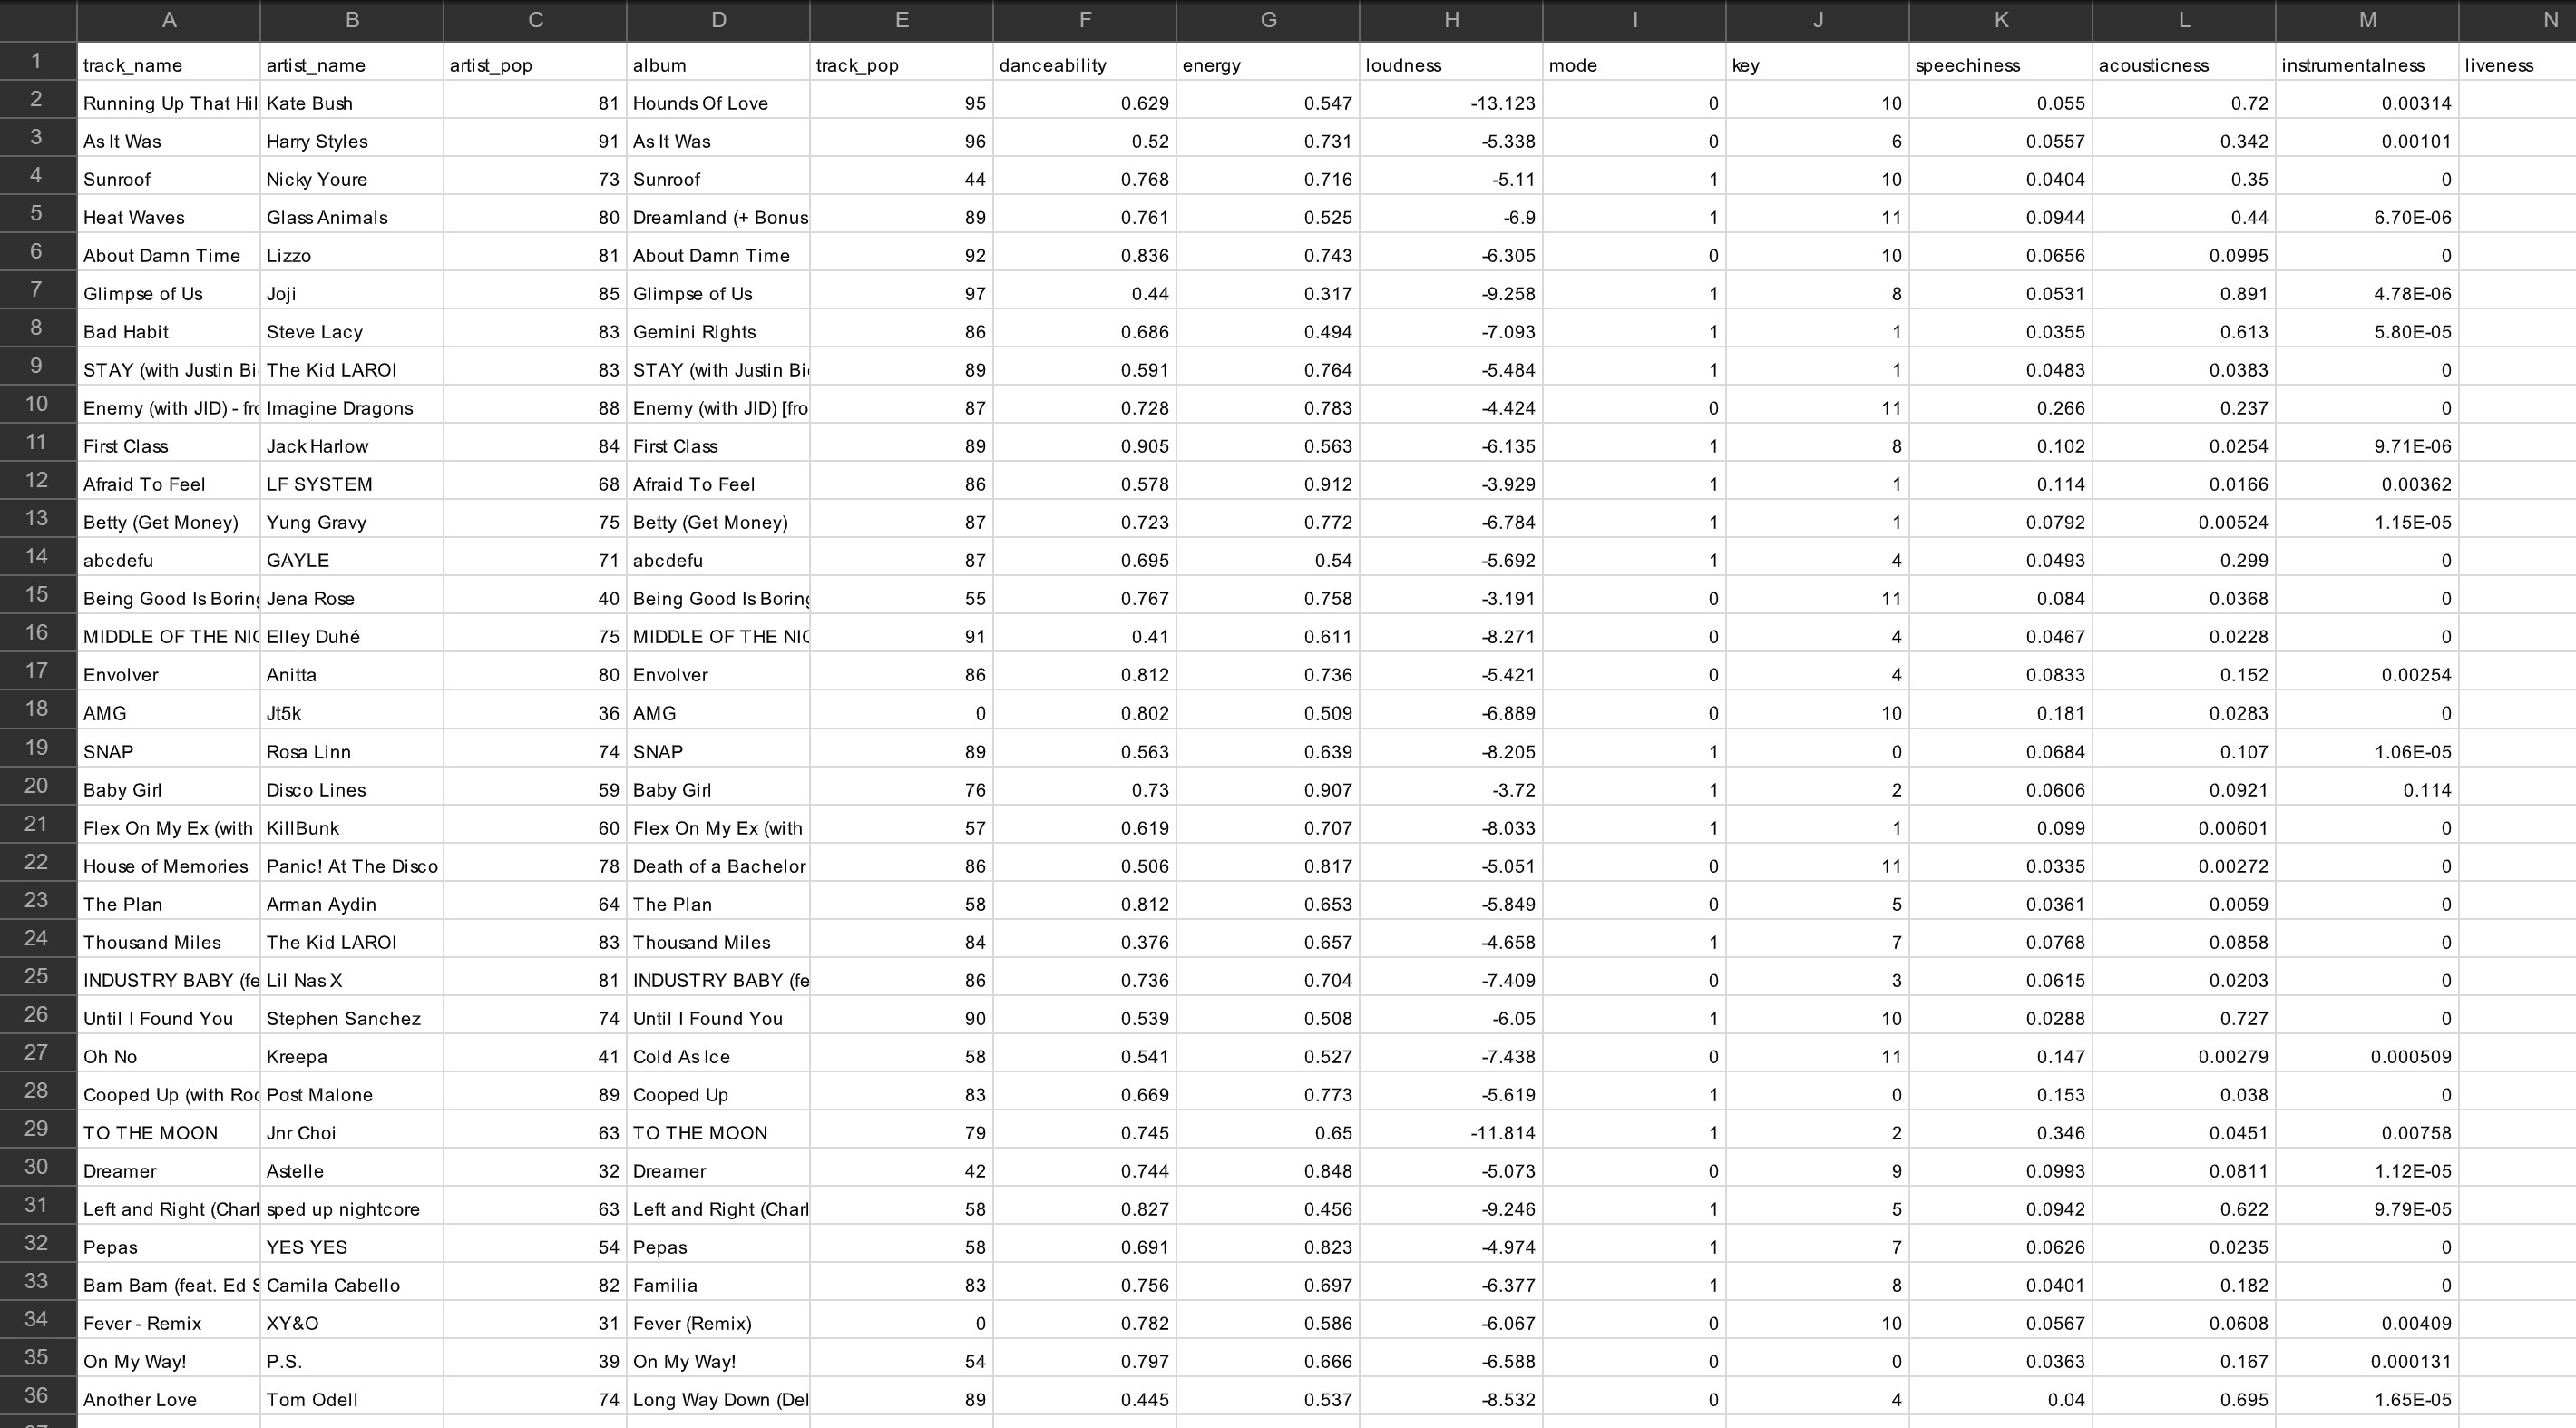
\includegraphics[width=5.86458in,height=\textheight]{images/tiktok_songs_screenshot.jpg}

}

\caption{Top Songs on TikTok}

\end{figure}%

\subsection{Billboard Dataset}

This dataset was found on Wikipedia. The table featured 3 columns and
100 observations. We used the importHTML function on Google Sheets to
convert the table on Wikipedia into a dataframe we could use. The grain
of the table is a song and its attributes. This table is different from
the TikTok and Spotify datasets in that it only has three columns: No.,
Title, and Artist(s). The No.~column represents the ranking of the
songs, with rankings spanning from 1 to 100.

\begin{figure}[H]

{\centering 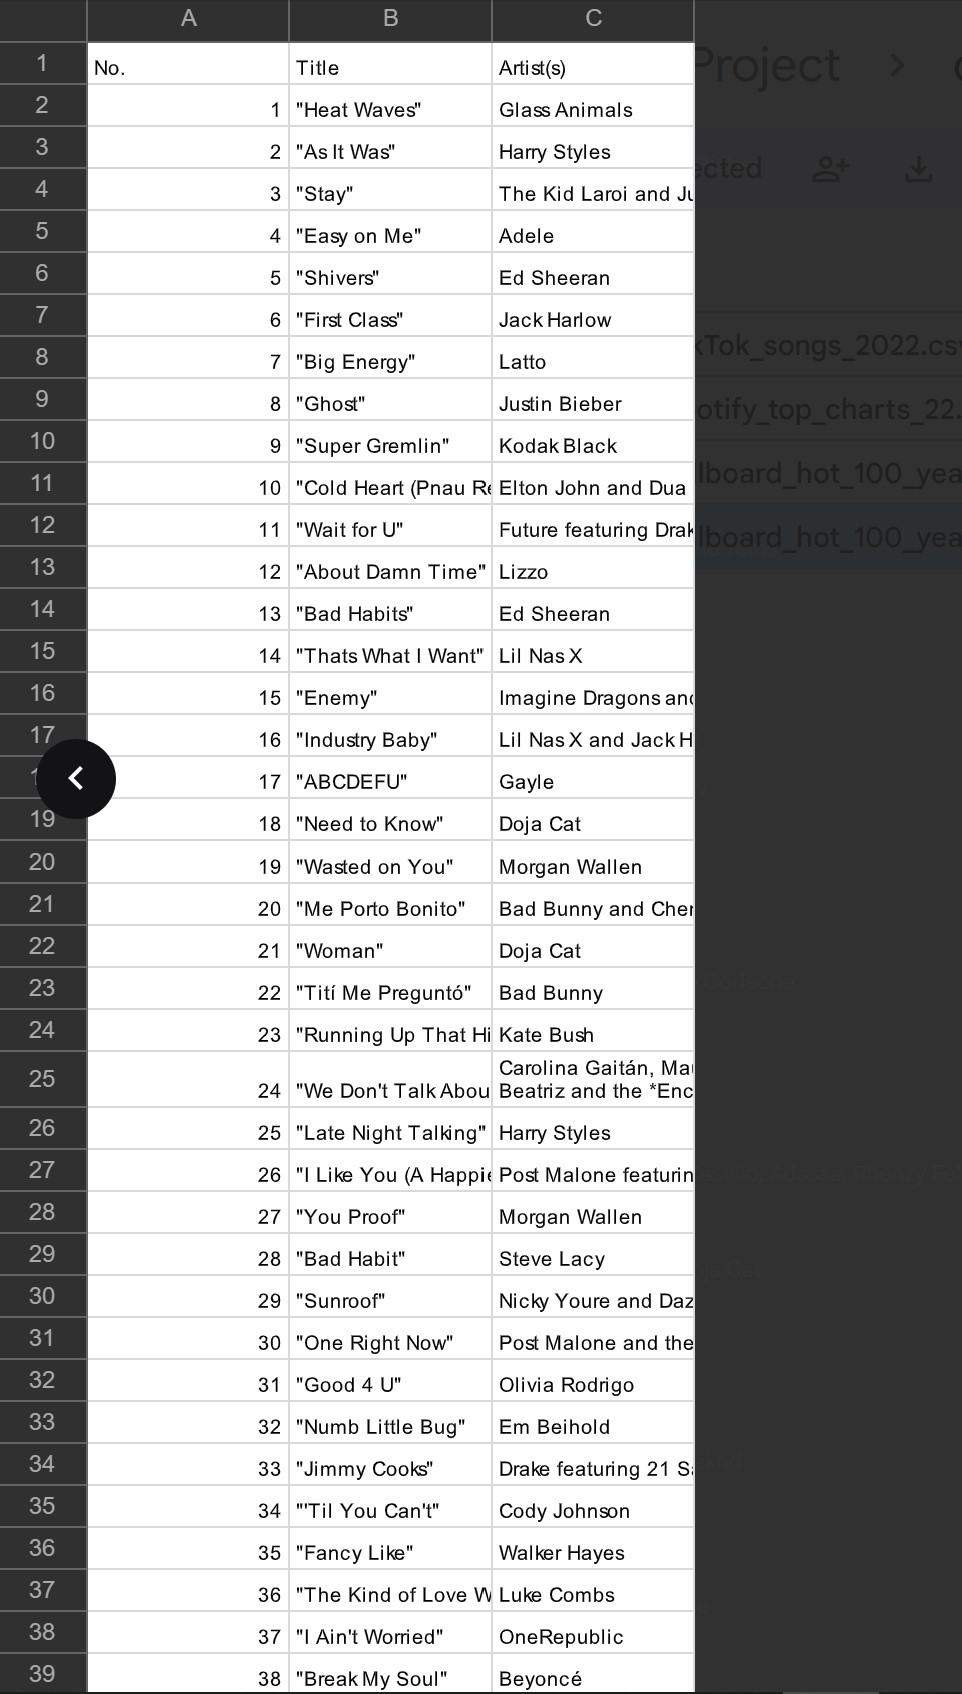
\includegraphics{images/billboard_screenshot.jpg}

}

\caption{Top Songs on Billboard Hot 100}

\end{figure}%

Both the Spotify and TikTok datasets have many extra columns that will
be unnecessary for the scope of this project. There are also variations
in the headers of the datasets and in the way that track names and
artist names are listed. The easiest way approach these datasets is to
eliminate the unnecessary columns and rename the headers so that the
datasets can be compared.

\bookmarksetup{startatroot}

\chapter*{Cleaning}\label{cleaning}
\addcontentsline{toc}{chapter}{Cleaning}

\markboth{Cleaning}{Cleaning}

Here is how we loaded and cleaned the data, and the problems that arose
in the process.

\begin{Shaded}
\begin{Highlighting}[]
\ImportTok{import}\NormalTok{ pandas }\ImportTok{as}\NormalTok{ pd}
\ImportTok{import}\NormalTok{ numpy }\ImportTok{as}\NormalTok{ np}
\end{Highlighting}
\end{Shaded}

\subsection*{Read}\label{read}
\addcontentsline{toc}{subsection}{Read}

\subsubsection{R}

These are the tables before cleaning and combining.

\begin{Shaded}
\begin{Highlighting}[]
\NormalTok{spotify\_top\_charts\_22 }\OtherTok{\textless{}{-}} \FunctionTok{read\_csv}\NormalTok{(}\StringTok{"spotify\_top\_charts\_22.csv"}\NormalTok{, }\AttributeTok{show\_col\_types =} \ConstantTok{FALSE}\NormalTok{)}
\NormalTok{TikTok\_songs\_2022 }\OtherTok{\textless{}{-}} \FunctionTok{read\_csv}\NormalTok{(}\StringTok{"TikTok\_songs\_2022.csv"}\NormalTok{, }\AttributeTok{show\_col\_types =} \ConstantTok{FALSE}\NormalTok{)}
\NormalTok{Billboard\_hot\_100\_year\_end\_2022 }\OtherTok{\textless{}{-}} \FunctionTok{read\_csv}\NormalTok{(}\StringTok{"Billboard\_hot\_100\_year\_end\_2022.csv"}\NormalTok{, }\AttributeTok{show\_col\_types =} \ConstantTok{FALSE}\NormalTok{)}
\end{Highlighting}
\end{Shaded}

\subsubsection{SQL}

These are the tables before cleaning and combining.

\begin{Shaded}
\begin{Highlighting}[]
\KeywordTok{CREATE} \KeywordTok{TABLE}\NormalTok{ spotify\_charts }\KeywordTok{AS}
  \KeywordTok{SELECT} \OperatorTok{*} \KeywordTok{FROM} \StringTok{\textquotesingle{}spotify\_top\_charts\_22.csv\textquotesingle{}}\NormalTok{;}
\KeywordTok{CREATE} \KeywordTok{TABLE}\NormalTok{ tiktok\_charts }\KeywordTok{AS}
  \KeywordTok{SELECT} \OperatorTok{*} \KeywordTok{FROM} \StringTok{\textquotesingle{}TikTok\_songs\_2022.csv\textquotesingle{}}\NormalTok{;}
\KeywordTok{CREATE} \KeywordTok{TABLE}\NormalTok{ billboard\_charts }\KeywordTok{AS}
  \KeywordTok{SELECT} \OperatorTok{*} \KeywordTok{FROM} \StringTok{\textquotesingle{}Billboard\_hot\_100\_year\_end\_2022.csv\textquotesingle{}}\NormalTok{;}
\end{Highlighting}
\end{Shaded}

\subsubsection{Python}

\begin{Shaded}
\begin{Highlighting}[]
\NormalTok{spotify\_top\_charts\_22 }\OperatorTok{=}\NormalTok{ pd.read\_csv(}\StringTok{"spotify\_top\_charts\_22.csv"}\NormalTok{)}
\NormalTok{TikTok\_songs\_2022 }\OperatorTok{=}\NormalTok{ pd.read\_csv(}\StringTok{"TikTok\_songs\_2022.csv"}\NormalTok{)}
\NormalTok{Billboard\_hot\_100\_year\_end\_2022 }\OperatorTok{=}\NormalTok{ pd.read\_csv(}\StringTok{"Billboard\_hot\_100\_year\_end\_2022.csv"}\NormalTok{)}
\end{Highlighting}
\end{Shaded}

All the datasets are messy. Both the Spotify and TikTok datasets have
columns that are not necessary for this project. To keep the tables
simple, we cleaned the data to make all three tables as similar as
possible. We renames all the columns holding the song title to
song\_title, the artist(s) artist, and the popularity/rank to
rank\_s/t/b for Spotify, TikTok, and Billboard, respectively. We also
included the tempo column on the Spotify and TikTok tables.

\subsection*{Cleaning}\label{cleaning-1}
\addcontentsline{toc}{subsection}{Cleaning}

\subsubsection*{Spotify}\label{spotify}
\addcontentsline{toc}{subsubsection}{Spotify}

\subsubsection{R}

For the Spotify data, we used select() to only keep the relevant
columns. We arranged the data so that the rows are listed with the more
popular songs near the top. The rank\_s column indicated the highest
rank the song appeared on the chart, so a lower number indicated that
the song was more popular.

\begin{Shaded}
\begin{Highlighting}[]
\NormalTok{spotify\_cleaned }\OtherTok{\textless{}{-}}\NormalTok{ spotify\_top\_charts\_22 }\SpecialCharTok{|\textgreater{}} 
  \FunctionTok{clean\_names}\NormalTok{() }\SpecialCharTok{|\textgreater{}} \CommentTok{\#clean the column headers}
  \FunctionTok{select}\NormalTok{(track\_name, artist\_names, peak\_rank, tempo) }\SpecialCharTok{|\textgreater{}} \CommentTok{\#filter only certain columns}
  \FunctionTok{rename}\NormalTok{(}\AttributeTok{song\_title =}\NormalTok{ track\_name, }\AttributeTok{artist =}\NormalTok{ artist\_names, }\AttributeTok{rank\_s =}\NormalTok{ peak\_rank) }\SpecialCharTok{|\textgreater{}} \CommentTok{\#rename the column headers}
  \FunctionTok{arrange}\NormalTok{(rank\_s) }\CommentTok{\#order from most to least popular}

\NormalTok{spotify\_cleaned}
\end{Highlighting}
\end{Shaded}

\begin{verbatim}
# A tibble: 646 x 4
   song_title                     artist                       rank_s tempo
   <chr>                          <chr>                         <dbl> <dbl>
 1 Heat Waves                     Glass Animals                     1  80.9
 2 STAY (with Justin Bieber)      The Kid LAROI, Justin Bieber      1 170. 
 3 abcdefu                        GAYLE                             1 122. 
 4 Easy On Me                     Adele                             1 142. 
 5 good 4 u                       Olivia Rodrigo                    1 167. 
 6 Blinding Lights                The Weeknd                        1 171. 
 7 MONTERO (Call Me By Your Name) Lil Nas X                         1 179. 
 8 drivers license                Olivia Rodrigo                    1 144. 
 9 DÁKITI                         Bad Bunny, Jhay Cortez            1 110. 
10 Beggin'                        Måneskin                          1 134. 
# i 636 more rows
\end{verbatim}

\subsubsection{SQL}

For the Spotify data, we used SELECT to only keep the relevant columns.
We arranged the data so that the rows are listed with the more popular
songs near the top. The rank\_s column indicated the highest rank the
song appeared on the chart, so a lower number indicated that the song
was more popular.

\begin{Shaded}
\begin{Highlighting}[]
\CommentTok{{-}{-}create a cleaned version of the spotify table and select only relevant columns}
\KeywordTok{CREATE} \KeywordTok{OR} \KeywordTok{REPLACE} \KeywordTok{TABLE}\NormalTok{ spotify\_cleaned }\KeywordTok{AS}
  \KeywordTok{SELECT}\NormalTok{ track\_name }\KeywordTok{AS}\NormalTok{ song\_title, artist\_names }\KeywordTok{AS}\NormalTok{ artist, peak\_rank }\KeywordTok{AS}\NormalTok{ rank\_s, tempo}
  \KeywordTok{FROM}\NormalTok{ spotify\_charts}
\NormalTok{;}
\CommentTok{{-}{-}order from most to least popular using the rank\_s column}
\KeywordTok{FROM}\NormalTok{ spotify\_cleaned}
\KeywordTok{ORDER} \KeywordTok{BY}\NormalTok{ rank\_s }\KeywordTok{ASC}
\end{Highlighting}
\end{Shaded}

\begin{longtable}[]{@{}
  >{\raggedright\arraybackslash}p{(\columnwidth - 6\tabcolsep) * \real{0.4133}}
  >{\raggedright\arraybackslash}p{(\columnwidth - 6\tabcolsep) * \real{0.3867}}
  >{\raggedleft\arraybackslash}p{(\columnwidth - 6\tabcolsep) * \real{0.0933}}
  >{\raggedleft\arraybackslash}p{(\columnwidth - 6\tabcolsep) * \real{0.1067}}@{}}
\caption{Displaying records 1 - 10}\tabularnewline
\toprule\noalign{}
\begin{minipage}[b]{\linewidth}\raggedright
song\_title
\end{minipage} & \begin{minipage}[b]{\linewidth}\raggedright
artist
\end{minipage} & \begin{minipage}[b]{\linewidth}\raggedleft
rank\_s
\end{minipage} & \begin{minipage}[b]{\linewidth}\raggedleft
tempo
\end{minipage} \\
\midrule\noalign{}
\endfirsthead
\toprule\noalign{}
\begin{minipage}[b]{\linewidth}\raggedright
song\_title
\end{minipage} & \begin{minipage}[b]{\linewidth}\raggedright
artist
\end{minipage} & \begin{minipage}[b]{\linewidth}\raggedleft
rank\_s
\end{minipage} & \begin{minipage}[b]{\linewidth}\raggedleft
tempo
\end{minipage} \\
\midrule\noalign{}
\endhead
\bottomrule\noalign{}
\endlastfoot
Heat Waves & Glass Animals & 1 & 80.870 \\
STAY (with Justin Bieber) & The Kid LAROI, Justin Bieber & 1 &
169.928 \\
abcdefu & GAYLE & 1 & 121.932 \\
Easy On Me & Adele & 1 & 141.981 \\
good 4 u & Olivia Rodrigo & 1 & 166.928 \\
Blinding Lights & The Weeknd & 1 & 171.005 \\
MONTERO (Call Me By Your Name) & Lil Nas X & 1 & 178.781 \\
drivers license & Olivia Rodrigo & 1 & 143.875 \\
DÁKITI & Bad Bunny, Jhay Cortez & 1 & 109.928 \\
Beggin' & Måneskin & 1 & 134.002 \\
\end{longtable}

\subsubsection{Python}

For the Spotify data, we used .filter to only keep the relevant columns.
We arranged the data so that the rows are listed with the more popular
songs near the top. The rank\_s column indicated the highest rank the
song appeared on the chart, so a lower number indicated that the song
was more popular.

\begin{Shaded}
\begin{Highlighting}[]
\NormalTok{spotify\_cleaned }\OperatorTok{=}\NormalTok{ (spotify\_top\_charts\_22}
\NormalTok{                   .}\BuiltInTok{filter}\NormalTok{(items }\OperatorTok{=}\NormalTok{ [}\StringTok{\textquotesingle{}track\_name\textquotesingle{}}\NormalTok{, }\StringTok{\textquotesingle{}artist\_names\textquotesingle{}}\NormalTok{, }\StringTok{\textquotesingle{}peak\_rank\textquotesingle{}}\NormalTok{, }\StringTok{\textquotesingle{}tempo\textquotesingle{}}\NormalTok{])}
\NormalTok{                   .rename(columns }\OperatorTok{=}\NormalTok{ \{}\StringTok{\textquotesingle{}track\_name\textquotesingle{}}\NormalTok{: }\StringTok{\textquotesingle{}song\_title\textquotesingle{}}\NormalTok{,}
                                      \StringTok{\textquotesingle{}artist\_names\textquotesingle{}}\NormalTok{: }\StringTok{\textquotesingle{}artist\textquotesingle{}}\NormalTok{,}
                                      \StringTok{\textquotesingle{}peak\_rank\textquotesingle{}}\NormalTok{: }\StringTok{\textquotesingle{}rank\_s\textquotesingle{}}\NormalTok{\})}
\NormalTok{                   .sort\_values(}\StringTok{\textquotesingle{}rank\_s\textquotesingle{}}\NormalTok{) }\CommentTok{\# lower number means higher rank}
\NormalTok{                  )}
\NormalTok{spotify\_cleaned}
\end{Highlighting}
\end{Shaded}

\begin{verbatim}
                              song_title  ...    tempo
0                             Heat Waves  ...   80.870
557                              HUMBLE.  ...  150.011
255                              Starboy  ...  186.003
246                     Call Out My Name  ...  134.170
207                        Glimpse of Us  ...  169.914
..                                   ...  ...      ...
500  Hold That Heat (feat. Travis Scott)  ...  130.045
561               Si Estuviésemos Juntos  ...  171.854
310                            Heartless  ...   87.999
583                       Paris to Tokyo  ...  146.733
609                            Sehnsucht  ...  142.090

[646 rows x 4 columns]
\end{verbatim}

\subsubsection*{TikTok}\label{tiktok}
\addcontentsline{toc}{subsubsection}{TikTok}

\subsubsection{R}

\begin{Shaded}
\begin{Highlighting}[]
\NormalTok{tiktok\_cleaned }\OtherTok{\textless{}{-}}\NormalTok{ TikTok\_songs\_2022 }\SpecialCharTok{|\textgreater{}}
  \FunctionTok{clean\_names}\NormalTok{() }\SpecialCharTok{|\textgreater{}} \CommentTok{\#clean the column headers}
  \FunctionTok{select}\NormalTok{(track\_name, artist\_name, track\_pop, tempo) }\SpecialCharTok{|\textgreater{}} \CommentTok{\#filter for certain columns}
  \FunctionTok{rename}\NormalTok{(}\AttributeTok{song\_title =}\NormalTok{ track\_name, }\AttributeTok{artist =}\NormalTok{ artist\_name, }\AttributeTok{rank\_t =}\NormalTok{ track\_pop) }\SpecialCharTok{|\textgreater{}} \CommentTok{\#rename the column headers}
  \FunctionTok{arrange}\NormalTok{(}\FunctionTok{desc}\NormalTok{(rank\_t)) }\CommentTok{\#arrange by popularity}
\NormalTok{tiktok\_cleaned}
\end{Highlighting}
\end{Shaded}

\begin{verbatim}
# A tibble: 263 x 4
   song_title                             artist            rank_t tempo
   <chr>                                  <chr>              <dbl> <dbl>
 1 Glimpse of Us                          Joji                  97  170.
 2 As It Was                              Harry Styles          96  174.
 3 Running Up That Hill (A Deal With God) Kate Bush             95  108.
 4 Late Night Talking                     Harry Styles          93  115.
 5 About Damn Time                        Lizzo                 92  109.
 6 Jimmy Cooks (feat. 21 Savage)          Drake                 92  166.
 7 MIDDLE OF THE NIGHT                    Elley Duhé            91  186.
 8 Until I Found You                      Stephen Sanchez       90  101.
 9 Blinding Lights                        The Weeknd            90  171.
10 Sweater Weather                        The Neighbourhood     90  124.
# i 253 more rows
\end{verbatim}

\subsubsection{SQL}

\begin{Shaded}
\begin{Highlighting}[]
\CommentTok{{-}{-}create a cleaned version of the tiktok table and select only relevant columns}
\KeywordTok{CREATE} \KeywordTok{OR} \KeywordTok{REPLACE} \KeywordTok{TABLE}\NormalTok{ tiktok\_cleaned }\KeywordTok{AS}
  \KeywordTok{SELECT}\NormalTok{ track\_name }\KeywordTok{AS}\NormalTok{ song\_title, artist\_name }\KeywordTok{AS}\NormalTok{ artist, track\_pop }\KeywordTok{AS}\NormalTok{ rank\_t, tempo}
  \KeywordTok{FROM}\NormalTok{ tiktok\_charts}
\NormalTok{;}
\CommentTok{{-}{-}order from most to least popular using the rank\_t column}
\KeywordTok{FROM}\NormalTok{ tiktok\_cleaned}
\KeywordTok{ORDER} \KeywordTok{BY}\NormalTok{ rank\_t }\KeywordTok{DESC}
\end{Highlighting}
\end{Shaded}

\begin{longtable}[]{@{}
  >{\raggedright\arraybackslash}p{(\columnwidth - 6\tabcolsep) * \real{0.5417}}
  >{\raggedright\arraybackslash}p{(\columnwidth - 6\tabcolsep) * \real{0.2500}}
  >{\raggedleft\arraybackslash}p{(\columnwidth - 6\tabcolsep) * \real{0.0972}}
  >{\raggedleft\arraybackslash}p{(\columnwidth - 6\tabcolsep) * \real{0.1111}}@{}}
\caption{Displaying records 1 - 10}\tabularnewline
\toprule\noalign{}
\begin{minipage}[b]{\linewidth}\raggedright
song\_title
\end{minipage} & \begin{minipage}[b]{\linewidth}\raggedright
artist
\end{minipage} & \begin{minipage}[b]{\linewidth}\raggedleft
rank\_t
\end{minipage} & \begin{minipage}[b]{\linewidth}\raggedleft
tempo
\end{minipage} \\
\midrule\noalign{}
\endfirsthead
\toprule\noalign{}
\begin{minipage}[b]{\linewidth}\raggedright
song\_title
\end{minipage} & \begin{minipage}[b]{\linewidth}\raggedright
artist
\end{minipage} & \begin{minipage}[b]{\linewidth}\raggedleft
rank\_t
\end{minipage} & \begin{minipage}[b]{\linewidth}\raggedleft
tempo
\end{minipage} \\
\midrule\noalign{}
\endhead
\bottomrule\noalign{}
\endlastfoot
Glimpse of Us & Joji & 97 & 169.914 \\
As It Was & Harry Styles & 96 & 173.930 \\
Running Up That Hill (A Deal With God) & Kate Bush & 95 & 108.375 \\
Late Night Talking & Harry Styles & 93 & 114.996 \\
About Damn Time & Lizzo & 92 & 108.966 \\
Jimmy Cooks (feat. 21 Savage) & Drake & 92 & 165.921 \\
MIDDLE OF THE NIGHT & Elley Duhé & 91 & 185.727 \\
Until I Found You & Stephen Sanchez & 90 & 101.358 \\
Blinding Lights & The Weeknd & 90 & 171.005 \\
Sweater Weather & The Neighbourhood & 90 & 124.053 \\
\end{longtable}

\subsubsection{Python}

\begin{Shaded}
\begin{Highlighting}[]
\NormalTok{tiktok\_cleaned }\OperatorTok{=}\NormalTok{ (TikTok\_songs\_2022}
\NormalTok{                   .}\BuiltInTok{filter}\NormalTok{(items }\OperatorTok{=}\NormalTok{ [}\StringTok{\textquotesingle{}track\_name\textquotesingle{}}\NormalTok{, }\StringTok{\textquotesingle{}artist\_name\textquotesingle{}}\NormalTok{, }\StringTok{\textquotesingle{}track\_pop\textquotesingle{}}\NormalTok{, }\StringTok{\textquotesingle{}tempo\textquotesingle{}}\NormalTok{])}
\NormalTok{                   .rename(columns }\OperatorTok{=}\NormalTok{ \{}\StringTok{\textquotesingle{}track\_name\textquotesingle{}}\NormalTok{: }\StringTok{\textquotesingle{}song\_title\textquotesingle{}}\NormalTok{,}
                                      \StringTok{\textquotesingle{}artist\_name\textquotesingle{}}\NormalTok{: }\StringTok{\textquotesingle{}artist\textquotesingle{}}\NormalTok{,}
                                      \StringTok{\textquotesingle{}track\_pop\textquotesingle{}}\NormalTok{: }\StringTok{\textquotesingle{}rank\_t\textquotesingle{}}\NormalTok{\})}
\NormalTok{                   .sort\_values(}\StringTok{\textquotesingle{}rank\_t\textquotesingle{}}\NormalTok{, ascending}\OperatorTok{=}\VariableTok{False}\NormalTok{) }\CommentTok{\# Higher number means higher ranking}
\NormalTok{                  )}
\NormalTok{tiktok\_cleaned}
\end{Highlighting}
\end{Shaded}

\begin{verbatim}
                                 song_title  ...    tempo
5                             Glimpse of Us  ...  169.914
1                                 As It Was  ...  173.930
0    Running Up That Hill (A Deal With God)  ...  108.375
52                       Late Night Talking  ...  114.996
260           Jimmy Cooks (feat. 21 Savage)  ...  165.921
..                                      ...  ...      ...
78             She Wolf (Falling to Pieces)  ...  125.030
75                         Looking for Love  ...  120.004
68                                     Lost  ...  123.070
184                            Backyard Boy  ...  138.026
131                                 What If  ...  126.001

[263 rows x 4 columns]
\end{verbatim}

\subsubsection*{Billboard}\label{billboard}
\addcontentsline{toc}{subsubsection}{Billboard}

\subsubsection{R}

\begin{Shaded}
\begin{Highlighting}[]
\NormalTok{billboard\_cleaned }\OtherTok{\textless{}{-}}\NormalTok{ Billboard\_hot\_100\_year\_end\_2022 }\SpecialCharTok{|\textgreater{}}
  \FunctionTok{clean\_names}\NormalTok{() }\SpecialCharTok{|\textgreater{}} \CommentTok{\#clean the column headers}
  \FunctionTok{select}\NormalTok{(title, artist\_s, no) }\SpecialCharTok{|\textgreater{}} \CommentTok{\#reorder the columns}
  \FunctionTok{rename}\NormalTok{(}\AttributeTok{song\_title =}\NormalTok{ title, }\AttributeTok{rank\_b =}\NormalTok{ no, }\AttributeTok{artist =}\NormalTok{ artist\_s) }\SpecialCharTok{|\textgreater{}} \CommentTok{\#rename the column headers}
  \FunctionTok{mutate}\NormalTok{(}\AttributeTok{song\_title =} \FunctionTok{str\_replace\_all}\NormalTok{(song\_title, }\StringTok{\textquotesingle{}"\textquotesingle{}}\NormalTok{, }\StringTok{\textquotesingle{}\textquotesingle{}}\NormalTok{)) }\CommentTok{\#take quotations off song titles}
\NormalTok{billboard\_cleaned}
\end{Highlighting}
\end{Shaded}

\begin{verbatim}
# A tibble: 100 x 3
   song_title              artist                          rank_b
   <chr>                   <chr>                            <dbl>
 1 Heat Waves              Glass Animals                        1
 2 As It Was               Harry Styles                         2
 3 Stay                    The Kid Laroi and Justin Bieber      3
 4 Easy on Me              Adele                                4
 5 Shivers                 Ed Sheeran                           5
 6 First Class             Jack Harlow                          6
 7 Big Energy              Latto                                7
 8 Ghost                   Justin Bieber                        8
 9 Super Gremlin           Kodak Black                          9
10 Cold Heart (Pnau Remix) Elton John and Dua Lipa             10
# i 90 more rows
\end{verbatim}

\subsubsection{SQL}

\begin{Shaded}
\begin{Highlighting}[]
\CommentTok{{-}{-}create a cleaned version of the billboard table and select only renamed relevant columns}
\KeywordTok{CREATE} \KeywordTok{OR} \KeywordTok{REPLACE} \KeywordTok{TABLE}\NormalTok{ billboard\_cleaned }\KeywordTok{AS}
  \KeywordTok{SELECT} \KeywordTok{replace}\NormalTok{(title, }\StringTok{\textquotesingle{}"\textquotesingle{}}\NormalTok{, }\StringTok{\textquotesingle{}\textquotesingle{}}\NormalTok{) }\KeywordTok{AS}\NormalTok{ song\_title, }\OtherTok{"artist(s)"} \KeywordTok{AS}\NormalTok{ artist, }\OtherTok{"no."} \KeywordTok{AS}\NormalTok{ rank\_b}
  \KeywordTok{FROM}\NormalTok{ billboard\_charts}
\NormalTok{;}
\CommentTok{{-}{-}order from most to least popular using the rank\_b column}
\KeywordTok{FROM}\NormalTok{ billboard\_cleaned}
\KeywordTok{ORDER} \KeywordTok{BY}\NormalTok{ rank\_b}
\end{Highlighting}
\end{Shaded}

\begin{longtable}[]{@{}llr@{}}
\caption{Displaying records 1 - 10}\tabularnewline
\toprule\noalign{}
song\_title & artist & rank\_b \\
\midrule\noalign{}
\endfirsthead
\toprule\noalign{}
song\_title & artist & rank\_b \\
\midrule\noalign{}
\endhead
\bottomrule\noalign{}
\endlastfoot
Heat Waves & Glass Animals & 1 \\
As It Was & Harry Styles & 2 \\
Stay & The Kid Laroi and Justin Bieber & 3 \\
Easy on Me & Adele & 4 \\
Shivers & Ed Sheeran & 5 \\
First Class & Jack Harlow & 6 \\
Big Energy & Latto & 7 \\
Ghost & Justin Bieber & 8 \\
Super Gremlin & Kodak Black & 9 \\
Cold Heart (Pnau Remix) & Elton John and Dua Lipa & 10 \\
\end{longtable}

\subsubsection{Python}

\begin{Shaded}
\begin{Highlighting}[]
\NormalTok{billboard\_cleaned }\OperatorTok{=}\NormalTok{ (Billboard\_hot\_100\_year\_end\_2022}
\NormalTok{                   .rename(columns }\OperatorTok{=}\NormalTok{ \{}\StringTok{\textquotesingle{}Title\textquotesingle{}}\NormalTok{: }\StringTok{\textquotesingle{}song\_title\textquotesingle{}}\NormalTok{,}
                                      \StringTok{\textquotesingle{}Artist(s)\textquotesingle{}}\NormalTok{: }\StringTok{\textquotesingle{}artist\textquotesingle{}}\NormalTok{,}
                                      \StringTok{\textquotesingle{}No.\textquotesingle{}}\NormalTok{: }\StringTok{\textquotesingle{}rank\_b\textquotesingle{}}\NormalTok{\})}
\NormalTok{                   .sort\_values(}\StringTok{\textquotesingle{}rank\_b\textquotesingle{}}\NormalTok{) }\CommentTok{\# highest to lowest rank}
\NormalTok{                  )}
\NormalTok{billboard\_cleaned[}\StringTok{\textquotesingle{}song\_title\textquotesingle{}}\NormalTok{] }\OperatorTok{=}\NormalTok{ billboard\_cleaned[}\StringTok{\textquotesingle{}song\_title\textquotesingle{}}\NormalTok{].}\BuiltInTok{str}\NormalTok{.replace(}\StringTok{\textquotesingle{}"\textquotesingle{}}\NormalTok{, }\StringTok{\textquotesingle{}\textquotesingle{}}\NormalTok{)}
\NormalTok{billboard\_cleaned}
\end{Highlighting}
\end{Shaded}

\begin{verbatim}
    rank_b                song_title                           artist
0        1                Heat Waves                    Glass Animals
1        2                 As It Was                     Harry Styles
2        3                      Stay  The Kid Laroi and Justin Bieber
3        4                Easy on Me                            Adele
4        5                   Shivers                       Ed Sheeran
..     ...                       ...                              ...
95      96              Flower Shops   Ernest featuring Morgan Wallen
96      97               To the Moon        Jnr Choi and Sam Tompkins
97      98                    Unholy         Sam Smith and Kim Petras
98      99           One Mississippi                       Kane Brown
99     100  Circles Around This Town                     Maren Morris

[100 rows x 3 columns]
\end{verbatim}

\subsection*{Challenges}\label{challenges}
\addcontentsline{toc}{subsection}{Challenges}

\subsubsection{R}

\begin{Shaded}
\begin{Highlighting}[]
\NormalTok{spotify\_cleaned }\SpecialCharTok{|\textgreater{}}
  \FunctionTok{filter}\NormalTok{(}\FunctionTok{str\_detect}\NormalTok{(song\_title, }\StringTok{\textquotesingle{}Enemy\textquotesingle{}}\NormalTok{)) }\CommentTok{\#filter for song titles containing "Enemy"}
\end{Highlighting}
\end{Shaded}

\begin{verbatim}
# A tibble: 2 x 4
  song_title                                                 artist rank_s tempo
  <chr>                                                      <chr>   <dbl> <dbl>
1 Enemy (with JID) - from the series Arcane League of Legen~ Imagi~      3  77.0
2 Enemy - From the series Arcane League of Legends           Imagi~    171  77.0
\end{verbatim}

\begin{Shaded}
\begin{Highlighting}[]
\NormalTok{tiktok\_cleaned }\SpecialCharTok{|\textgreater{}}
  \FunctionTok{filter}\NormalTok{(}\FunctionTok{str\_detect}\NormalTok{(song\_title, }\StringTok{\textquotesingle{}Enemy\textquotesingle{}}\NormalTok{))}
\end{Highlighting}
\end{Shaded}

\begin{verbatim}
# A tibble: 1 x 4
  song_title                                                 artist rank_t tempo
  <chr>                                                      <chr>   <dbl> <dbl>
1 Enemy (with JID) - from the series Arcane League of Legen~ Imagi~     87  77.0
\end{verbatim}

\begin{Shaded}
\begin{Highlighting}[]
\NormalTok{billboard\_cleaned }\SpecialCharTok{|\textgreater{}}
  \FunctionTok{filter}\NormalTok{(}\FunctionTok{str\_detect}\NormalTok{(song\_title, }\StringTok{\textquotesingle{}Enemy\textquotesingle{}}\NormalTok{))}
\end{Highlighting}
\end{Shaded}

\begin{verbatim}
# A tibble: 1 x 3
  song_title artist                  rank_b
  <chr>      <chr>                    <dbl>
1 Enemy      Imagine Dragons and JID     15
\end{verbatim}

\subsubsection{SQL}

\begin{Shaded}
\begin{Highlighting}[]
\KeywordTok{SELECT} \OperatorTok{*}
\KeywordTok{FROM}\NormalTok{ spotify\_cleaned}
\KeywordTok{WHERE}\NormalTok{ song\_title }\KeywordTok{LIKE} \StringTok{\textquotesingle{}\%Enemy\%\textquotesingle{}}
\end{Highlighting}
\end{Shaded}

\begin{longtable}[]{@{}
  >{\raggedright\arraybackslash}p{(\columnwidth - 6\tabcolsep) * \real{0.4918}}
  >{\raggedright\arraybackslash}p{(\columnwidth - 6\tabcolsep) * \real{0.3934}}
  >{\raggedleft\arraybackslash}p{(\columnwidth - 6\tabcolsep) * \real{0.0574}}
  >{\raggedleft\arraybackslash}p{(\columnwidth - 6\tabcolsep) * \real{0.0574}}@{}}
\caption{2 records}\tabularnewline
\toprule\noalign{}
\begin{minipage}[b]{\linewidth}\raggedright
song\_title
\end{minipage} & \begin{minipage}[b]{\linewidth}\raggedright
artist
\end{minipage} & \begin{minipage}[b]{\linewidth}\raggedleft
rank\_s
\end{minipage} & \begin{minipage}[b]{\linewidth}\raggedleft
tempo
\end{minipage} \\
\midrule\noalign{}
\endfirsthead
\toprule\noalign{}
\begin{minipage}[b]{\linewidth}\raggedright
song\_title
\end{minipage} & \begin{minipage}[b]{\linewidth}\raggedright
artist
\end{minipage} & \begin{minipage}[b]{\linewidth}\raggedleft
rank\_s
\end{minipage} & \begin{minipage}[b]{\linewidth}\raggedleft
tempo
\end{minipage} \\
\midrule\noalign{}
\endhead
\bottomrule\noalign{}
\endlastfoot
Enemy (with JID) - from the series Arcane League of Legends & Imagine
Dragons, JID, Arcane, League of Legends & 3 & 77.011 \\
Enemy - From the series Arcane League of Legends & Imagine Dragons,
Arcane, League of Legends & 171 & 77.029 \\
\end{longtable}

\begin{Shaded}
\begin{Highlighting}[]
\KeywordTok{SELECT} \OperatorTok{*}
\KeywordTok{FROM}\NormalTok{ tiktok\_cleaned}
\KeywordTok{WHERE}\NormalTok{ song\_title }\KeywordTok{LIKE} \StringTok{\textquotesingle{}\%Enemy\%\textquotesingle{}}
\end{Highlighting}
\end{Shaded}

\begin{longtable}[]{@{}
  >{\raggedright\arraybackslash}p{(\columnwidth - 6\tabcolsep) * \real{0.6667}}
  >{\raggedright\arraybackslash}p{(\columnwidth - 6\tabcolsep) * \real{0.1778}}
  >{\raggedleft\arraybackslash}p{(\columnwidth - 6\tabcolsep) * \real{0.0778}}
  >{\raggedleft\arraybackslash}p{(\columnwidth - 6\tabcolsep) * \real{0.0778}}@{}}
\caption{1 records}\tabularnewline
\toprule\noalign{}
\begin{minipage}[b]{\linewidth}\raggedright
song\_title
\end{minipage} & \begin{minipage}[b]{\linewidth}\raggedright
artist
\end{minipage} & \begin{minipage}[b]{\linewidth}\raggedleft
rank\_t
\end{minipage} & \begin{minipage}[b]{\linewidth}\raggedleft
tempo
\end{minipage} \\
\midrule\noalign{}
\endfirsthead
\toprule\noalign{}
\begin{minipage}[b]{\linewidth}\raggedright
song\_title
\end{minipage} & \begin{minipage}[b]{\linewidth}\raggedright
artist
\end{minipage} & \begin{minipage}[b]{\linewidth}\raggedleft
rank\_t
\end{minipage} & \begin{minipage}[b]{\linewidth}\raggedleft
tempo
\end{minipage} \\
\midrule\noalign{}
\endhead
\bottomrule\noalign{}
\endlastfoot
Enemy (with JID) - from the series Arcane League of Legends & Imagine
Dragons & 87 & 77.011 \\
\end{longtable}

\begin{Shaded}
\begin{Highlighting}[]
\KeywordTok{SELECT} \OperatorTok{*}
\KeywordTok{FROM}\NormalTok{ billboard\_cleaned}
\KeywordTok{WHERE}\NormalTok{ song\_title }\KeywordTok{LIKE} \StringTok{\textquotesingle{}\%Enemy\%\textquotesingle{}}
\end{Highlighting}
\end{Shaded}

\begin{longtable}[]{@{}llr@{}}
\caption{1 records}\tabularnewline
\toprule\noalign{}
song\_title & artist & rank\_b \\
\midrule\noalign{}
\endfirsthead
\toprule\noalign{}
song\_title & artist & rank\_b \\
\midrule\noalign{}
\endhead
\bottomrule\noalign{}
\endlastfoot
Enemy & Imagine Dragons and JID & 15 \\
\end{longtable}

\subsubsection{Python V1}

\begin{Shaded}
\begin{Highlighting}[]
\BuiltInTok{print}\NormalTok{(spotify\_cleaned[spotify\_cleaned[}\StringTok{\textquotesingle{}song\_title\textquotesingle{}}\NormalTok{].}\BuiltInTok{str}\NormalTok{.contains(}\StringTok{"Enemy"}\NormalTok{)])}
\end{Highlighting}
\end{Shaded}

\begin{verbatim}
                                            song_title  ...   tempo
3    Enemy (with JID) - from the series Arcane Leag...  ...  77.011
380   Enemy - From the series Arcane League of Legends  ...  77.029

[2 rows x 4 columns]
\end{verbatim}

\begin{Shaded}
\begin{Highlighting}[]
\BuiltInTok{print}\NormalTok{(tiktok\_cleaned[tiktok\_cleaned[}\StringTok{\textquotesingle{}song\_title\textquotesingle{}}\NormalTok{].}\BuiltInTok{str}\NormalTok{.contains(}\StringTok{"Enemy"}\NormalTok{)])}
\end{Highlighting}
\end{Shaded}

\begin{verbatim}
                                          song_title  ...   tempo
8  Enemy (with JID) - from the series Arcane Leag...  ...  77.011

[1 rows x 4 columns]
\end{verbatim}

\begin{Shaded}
\begin{Highlighting}[]
\BuiltInTok{print}\NormalTok{(billboard\_cleaned[billboard\_cleaned[}\StringTok{\textquotesingle{}song\_title\textquotesingle{}}\NormalTok{].}\BuiltInTok{str}\NormalTok{.contains(}\StringTok{"Enemy"}\NormalTok{)])}
\end{Highlighting}
\end{Shaded}

\begin{verbatim}
    rank_b song_title                   artist
14      15      Enemy  Imagine Dragons and JID
\end{verbatim}

\subsubsection{Python V2}

\begin{Shaded}
\begin{Highlighting}[]
\BuiltInTok{print}\NormalTok{(spotify\_cleaned.query(}\StringTok{\textquotesingle{}song\_title.str.contains("Enemy")\textquotesingle{}}\NormalTok{, engine}\OperatorTok{=}\StringTok{\textquotesingle{}python\textquotesingle{}}\NormalTok{))}
\end{Highlighting}
\end{Shaded}

\begin{verbatim}
                                            song_title  ...   tempo
3    Enemy (with JID) - from the series Arcane Leag...  ...  77.011
380   Enemy - From the series Arcane League of Legends  ...  77.029

[2 rows x 4 columns]
\end{verbatim}

\begin{Shaded}
\begin{Highlighting}[]
\BuiltInTok{print}\NormalTok{(tiktok\_cleaned.query(}\StringTok{\textquotesingle{}song\_title.str.contains("Enemy")\textquotesingle{}}\NormalTok{, engine}\OperatorTok{=}\StringTok{\textquotesingle{}python\textquotesingle{}}\NormalTok{))}
\end{Highlighting}
\end{Shaded}

\begin{verbatim}
                                          song_title  ...   tempo
8  Enemy (with JID) - from the series Arcane Leag...  ...  77.011

[1 rows x 4 columns]
\end{verbatim}

\begin{Shaded}
\begin{Highlighting}[]
\BuiltInTok{print}\NormalTok{(billboard\_cleaned.query(}\StringTok{\textquotesingle{}song\_title.str.contains("Enemy")\textquotesingle{}}\NormalTok{, engine}\OperatorTok{=}\StringTok{\textquotesingle{}python\textquotesingle{}}\NormalTok{))}
\end{Highlighting}
\end{Shaded}

\begin{verbatim}
    rank_b song_title                   artist
14      15      Enemy  Imagine Dragons and JID
\end{verbatim}

All three charts record the song title differently. The Spotify chart
has two different versions of ``Enemy'' on it: one with JID and one
without. The TikTok and Billboard charts both have the version with JID,
but the name of the song and and artists listed are different. To handle
these synonyms, we created a lookup dictionary and applied it to each
dataframe. We chose to apply the dictionary to each individual table
rather than a combined table so that when we combine the tables, songs
with the same title and artists would be combined. The dictionaries for
the song titles and artist names were created in Google Sheets and
uploaded to RStudio as csv files.

\subsection*{}\label{section}
\addcontentsline{toc}{subsection}{}

\subsubsection{R}

\begin{Shaded}
\begin{Highlighting}[]
\NormalTok{song\_title\_lookup }\OtherTok{\textless{}{-}} \FunctionTok{read\_csv}\NormalTok{(}\StringTok{"dict\_song\_titles.csv"}\NormalTok{, }\AttributeTok{show\_col\_types =} \ConstantTok{FALSE}\NormalTok{)}
\NormalTok{song\_title\_lookup}
\end{Highlighting}
\end{Shaded}

\begin{verbatim}
# A tibble: 4 x 2
  canonical_name                                              alt_name          
  <chr>                                                       <chr>             
1 Enemy (with JID) - from the series Arcane League of Legends Enemy             
2 BREAK MY SOUL                                               Break My Soul     
3 MAMIII                                                      Mamii             
4 Bam Bam                                                     Bam Bam (feat. Ed~
\end{verbatim}

\begin{Shaded}
\begin{Highlighting}[]
\NormalTok{spotify\_cleaned }\OtherTok{\textless{}{-}}\NormalTok{ spotify\_cleaned }\SpecialCharTok{|\textgreater{}}
  \FunctionTok{left\_join}\NormalTok{(song\_title\_lookup, }\AttributeTok{by =} \FunctionTok{join\_by}\NormalTok{(song\_title }\SpecialCharTok{==}\NormalTok{ alt\_name)) }\SpecialCharTok{|\textgreater{}} \CommentTok{\#join the Spotify table and dictionary table on song\_title and alt\_name, making a new column called "canonical\_name" in the Spotify table}
  \FunctionTok{mutate}\NormalTok{(}\AttributeTok{song\_title =} \FunctionTok{coalesce}\NormalTok{(canonical\_name, song\_title)) }\SpecialCharTok{|\textgreater{}} \CommentTok{\#coalesce takes the first non{-}null value}
  \FunctionTok{select}\NormalTok{(song\_title, artist, rank\_s, tempo) }\CommentTok{\#keep only relevant columns}
\end{Highlighting}
\end{Shaded}

\begin{Shaded}
\begin{Highlighting}[]
\NormalTok{tiktok\_cleaned }\OtherTok{\textless{}{-}}\NormalTok{ tiktok\_cleaned }\SpecialCharTok{|\textgreater{}}
  \FunctionTok{left\_join}\NormalTok{(song\_title\_lookup, }\AttributeTok{by =} \FunctionTok{join\_by}\NormalTok{(song\_title }\SpecialCharTok{==}\NormalTok{ alt\_name)) }\SpecialCharTok{|\textgreater{}}
  \FunctionTok{mutate}\NormalTok{(}\AttributeTok{song\_title =} \FunctionTok{coalesce}\NormalTok{(canonical\_name, song\_title)) }\SpecialCharTok{|\textgreater{}} \CommentTok{\#coalesce takes the first non{-}null value}
  \FunctionTok{select}\NormalTok{(song\_title, artist, rank\_t, tempo)}
\end{Highlighting}
\end{Shaded}

\begin{Shaded}
\begin{Highlighting}[]
\NormalTok{billboard\_cleaned }\OtherTok{\textless{}{-}}\NormalTok{ billboard\_cleaned }\SpecialCharTok{|\textgreater{}}
  \FunctionTok{left\_join}\NormalTok{(song\_title\_lookup, }\AttributeTok{by =} \FunctionTok{join\_by}\NormalTok{(song\_title }\SpecialCharTok{==}\NormalTok{ alt\_name)) }\SpecialCharTok{|\textgreater{}} \CommentTok{\#join the Spotify table and dictionary table on song\_title and alt\_name, making a new column called "canonical\_name" in the Spotify table}
  \FunctionTok{mutate}\NormalTok{(}\AttributeTok{song\_title =} \FunctionTok{coalesce}\NormalTok{(canonical\_name, song\_title)) }\SpecialCharTok{|\textgreater{}} \CommentTok{\#coalesce takes the first non{-}null value}
  \FunctionTok{select}\NormalTok{(song\_title, artist, rank\_b) }\CommentTok{\#keep only relevant columns}
\end{Highlighting}
\end{Shaded}

\subsubsection{SQL}

\subsubsection{Python}




\end{document}
